\section{Mesin Enigma}
\label{sec:enigma}

Enigma adalah mesin enkripsi elektromekanik untuk melakukan enkripsi dan
dekripsi. Mesin ini ditemukan dan dipatenkan oleh insinyur Jerman, Arthur
Scherbius, untuk tujuan komersial, diplomatik, dan militer. Enigma menjadi
terkenal karena dipakai oleh tentara Nazi Jerman selama Perang Dunia II untuk
mengenkripsi pesan-pesan militer. Nama Enigma berasal dari bahasa Latin
\textit{enigmae}, yang berarti teka-teki.

\subsection{Komponen Mesin}

Enigma memiliki papan tombol (\textit{keyboard}) untuk mengetik pesan. Papan
lampu (\textit{lampboard}) menunjukkan huruf cipherteks yang dihasilkan.
Operator mengetik huruf plainteks pada keyboard, lalu menyalin huruf
cipherteks yang menyala pada lampboard. Cipherteks itu kemudian dikirim ke
penerima pesan.

Enigma menggunakan rotor, yaitu roda berputar yang membentuk huruf cipherteks
yang berubah-ubah. Mesin ini memiliki tiga rotor, dan kemudian empat rotor.
Posisi rotor mengendalikan penyandian setiap huruf. Papan steker
(\textit{plugboard}) menukar pasangan huruf, dan setelannya diubah setiap
hari. Reflektor memantulkan sinyal di dalam mesin. Jendela pengamat
menunjukkan posisi setiap rotor. Bagian-bagian itu diperlihatkan pada
Gambar~\ref{fig:enigma-bagian}.

\begin{figure}[htbp]
    \centering
    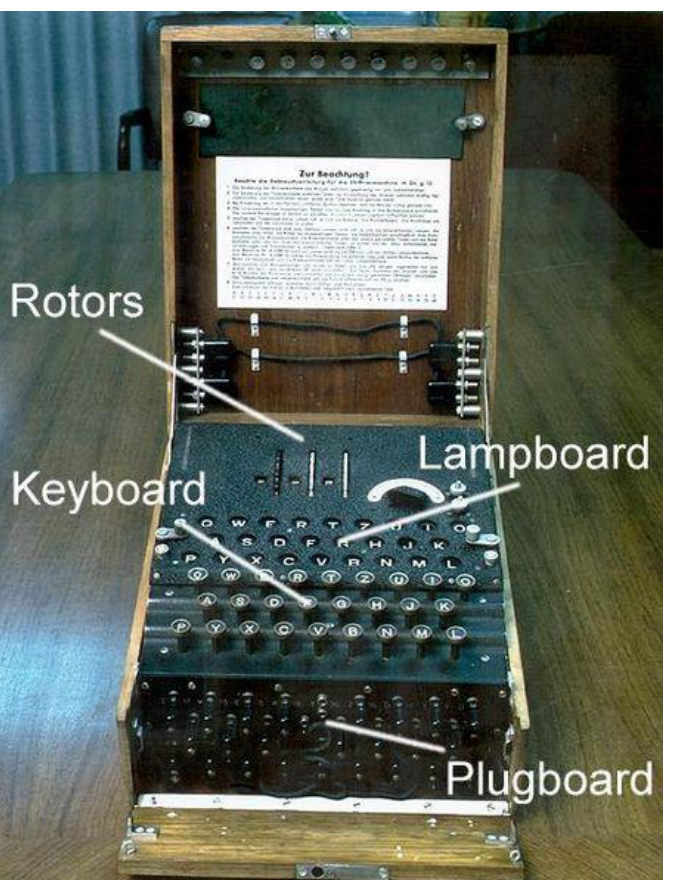
\includegraphics[width=0.65\linewidth, height=0.5\textheight, keepaspectratio]{figures/enigma-bagian.png}
    \caption{Mesin Enigma beserta rotor, papan tombol, papan lampu, dan papan steker}
    \label{fig:enigma-bagian}
    \sumber{Munir, \textit{IF4020 Kriptografi}, ITB.}
\end{figure}

\subsection{Mekanisme Rotor}

Setiap rotor melakukan substitusi abjad-tunggal. Hasil substitusi oleh suatu
rotor menjadi huruf masukan untuk rotor berikutnya. Hasil substitusi oleh
rotor terakhir menjadi huruf cipherteks. Setiap kali sebuah huruf dienkripsi
oleh sebuah rotor, rotor berputar satu huruf. Dengan demikian, huruf plainteks
berikutnya memperoleh substitusi yang baru.

Setelah berputar 26 huruf, rotor kembali pada posisi semula. Jadi Enigma
adalah cipher abjad-majemuk dengan periode 26 untuk satu rotor. Setiap kali
rotor pertama selesai bergeser 26 kali, rotor kedua bergeser satu huruf.
Setelah rotor kedua bergeser 26 kali, rotor ketiga bergeser satu huruf.
Demikian seterusnya seperti odometer. Pergeseran rotor kanan diperlihatkan
pada Gambar~\ref{fig:enigma-skema}.

\begin{figure}[htbp]
    \centering
    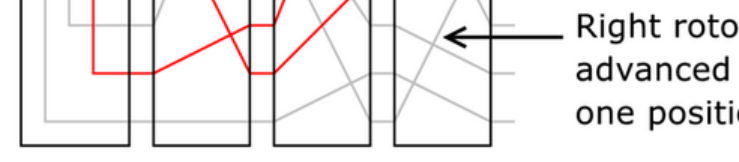
\includegraphics[width=0.95\linewidth, height=0.2\textheight, keepaspectratio]{figures/enigma-skema.png}
    \caption{Rotor kanan bergeser satu posisi setelah sebuah huruf dienkripsi}
    \label{fig:enigma-skema}
    \sumber{Munir, \textit{IF4020 Kriptografi}, ITB.}
\end{figure}

Mesin Enigma ada yang memakai tiga rotor dan ada yang memakai empat rotor.
Untuk mesin empat rotor, ada
\[
26 \times 26 \times 26 \times 26 = 456.976
\]
kemungkinan huruf cipherteks sebelum urutan cipherteks berulang. Posisi awal
keempat rotor dapat diatur. Posisi awal itulah yang menjadi kunci Enigma.

\subsection{Contoh Enkripsi Huruf Demi Huruf}

Misalkan tiga rotor disederhanakan menjadi alfabet enam huruf. Huruf plainteks
\code{D} ditekan pada keyboard. Rotor pertama mengenkripsinya menjadi
\code{E}. Huruf \code{E} menjadi masukan rotor kedua dan dienkripsi menjadi
\code{B}. Huruf \code{B} menjadi masukan rotor ketiga dan dienkripsi menjadi
\code{E}. Jadi, huruf \code{D} dienkripsi menjadi \code{E}. Setelah itu, rotor
ketiga bergeser satu huruf. Jika \code{D} dienkripsi kembali, hasilnya adalah
\code{A}. Proses itu diperlihatkan pada Gambar~\ref{fig:enigma-rotor}.

\begin{figure}[htbp]
    \centering
    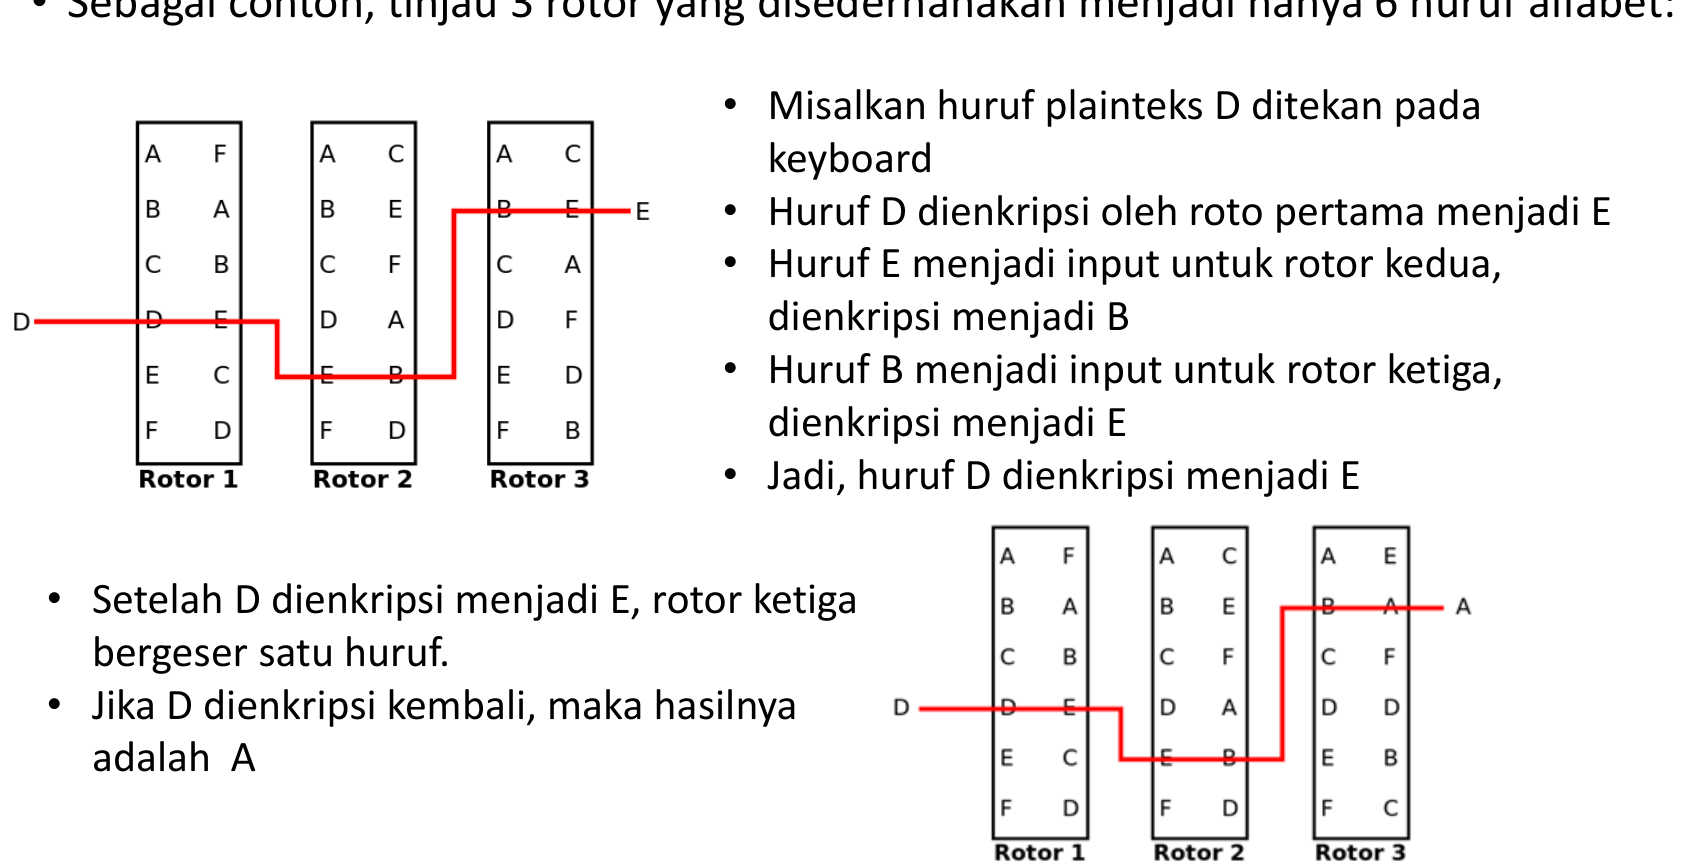
\includegraphics[width=0.95\linewidth, height=0.4\textheight, keepaspectratio]{figures/enigma-rotor.png}
    \caption{Enkripsi huruf \code{D} melalui tiga rotor beralfabet enam huruf}
    \label{fig:enigma-rotor}
    \sumber{Munir, \textit{IF4020 Kriptografi}, ITB.}
\end{figure}

Pada mesin yang sesungguhnya, jalur sinyal melewati papan steker, tiga rotor,
reflektor, lalu kembali melalui ketiga rotor dan papan steker. Tabel berikut
memperlihatkan rincian untuk tiga huruf pertama dari pesan
\code{PESAWATMENDARAT}. Pesan itu menghasilkan cipherteks
\code{GUFYLFRKQEJXVHM}. Rincian jalur sinyalnya ada pada
Tabel~\ref{tab:enigma-langkah}.

\begin{table}[htbp]
\centering
\small
\begin{tabularx}{\linewidth}{@{}c c >{\raggedright\arraybackslash}X c@{}}
\hline
Huruf & Posisi rotor & Jalur sinyal & Keluaran \\
\hline
\code{P} & \texttt{ABE} & steker \code{P} $\rightarrow$ R3 \code{W}
$\rightarrow$ R2 \code{U} $\rightarrow$ R1 \code{A} $\rightarrow$ reflektor
\code{Y} $\rightarrow$ R1 \code{O} $\rightarrow$ R2 \code{T} $\rightarrow$ R3
\code{G} $\rightarrow$ steker \code{G} & \textbf{\code{G}} \\[3pt]
\code{E} & \texttt{ABM} & steker \code{E} $\rightarrow$ R3 \code{W}
$\rightarrow$ R2 \code{U} $\rightarrow$ R1 \code{A} $\rightarrow$ reflektor
\code{Y} $\rightarrow$ R1 \code{O} $\rightarrow$ R2 \code{T} $\rightarrow$ R3
\code{Q} $\rightarrow$ steker \code{Q} & \textbf{\code{Q}} \\[3pt]
\code{S} & \texttt{ABG} & steker \code{S} $\rightarrow$ R3 \code{K}
$\rightarrow$ R2 \code{G} $\rightarrow$ R1 \code{D} $\rightarrow$ reflektor
\code{H} $\rightarrow$ R1 \code{P} $\rightarrow$ R2 \code{P} $\rightarrow$ R3
\code{F} $\rightarrow$ steker \code{F} & \textbf{\code{F}} \\
\hline
\end{tabularx}
\caption{Jalur enkripsi tiga huruf pertama pesan Enigma}
\label{tab:enigma-langkah}
\sumber{Data dari Munir, \textit{IF4020 Kriptografi}, ITB.}
\end{table}

\subsection{Kriptanalisis Enigma}

Kriptanalisis mesin Enigma pertama kali ditemukan pada tahun 1932 oleh tiga
kriptografer Polandia, yaitu Marian Rejewski, Jerzy R\'o\.zycki, dan Henryk
Zygalski. Pemerintahan Nazi Jerman kemudian mendesain ulang mesin Enigma pada
tahun 1939. Desain baru menambahkan papan steker dan reflektor, sehingga proses
enkripsi menjadi lebih kompleks. Metode kriptanalisis Enigma sebelumnya tidak
dapat digunakan lagi.

Dengan bantuan Polandia, Prancis, dan Inggris, dibuat mesin pemecah Enigma
yang baru. Mesin itu diberi nama \textit{bombe} dan dirancang oleh Alan
Turing. \textit{Bombe} berhasil memecahkan Enigma cipher buatan Jerman.
Keberhasilan itu dianggap sebagai faktor yang memperpendek Perang Dunia II
menjadi hanya dua tahun. Mesin \textit{bombe} diperlihatkan pada
Gambar~\ref{fig:enigma-bombe}.

\begin{figure}[htbp]
    \centering
    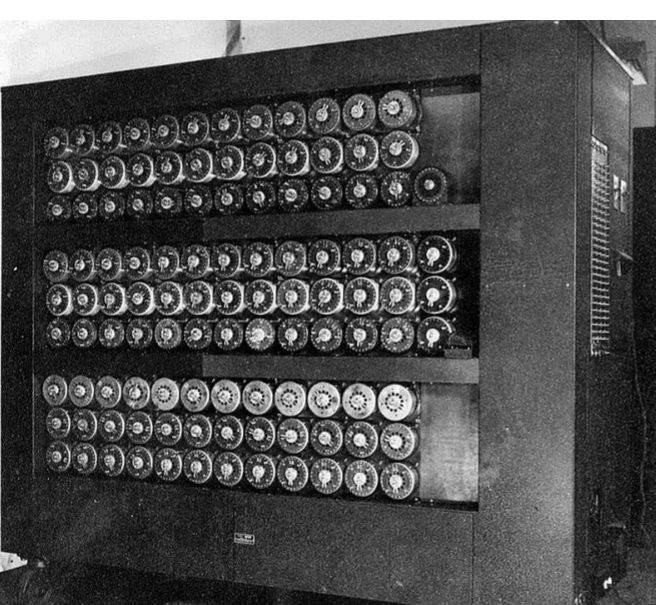
\includegraphics[width=0.55\linewidth, height=0.45\textheight, keepaspectratio]{figures/enigma-bombe.png}
    \caption{Mesin \textit{bombe} yang dirancang oleh Alan Turing}
    \label{fig:enigma-bombe}
    \sumber{Munir, \textit{IF4020 Kriptografi}, ITB.}
\end{figure}
